%!TEX root = ../main.tex

% \part{Enhancing the System Stability Assessment}

%%%%%%%%%%%%%%%%%%%%%%%%%%%%%%%
%%%%%%%%%%%%%%%%%%%%%%%%%%%%%%%
\chapter{Validation Setup and Results}
\label{chap:verification}

\begin{textblock*}{.7\textwidth}(70mm-\offset,25mm-\offset)
    \begin{fquote}[Mark Twain]
        If you tell the truth, you don't have to remember anything.
    \end{fquote}
\end{textblock*}

%%%%%%%%%%%%%%%%%%%%%%%%%%%%%%%
\section{Representative Electrical Networks}
\label{sec:networks}

The following section shall introduce the used power systems in the simulation with the Python framework, considering verification, and also extension meaning the performed case studies in \autoref{chap:case-study}. 
The models are chosen to represent different network sizes and complexities, thus allowing the objective of graded interaction levels of the developed (transformer) model. 
The models are based on the work of \textcite{machowski_2020}, \textcite{kundur_2022}, \textcite{IEEELoadModeling_2022}, and \textcite{vancutsem_2020}.
On important note to take for all the presented networks in the following, is the consequent absence of machine control units. 
Only where mentioned explicitly, they are used.

\subsubsection{Single Machine Infinite Bus (SMIB) Model}

One very popular and thus powerful electrical network for the verification of power system stability is the \acs{SMIB} model. 
It is a compact and simplified model of a power system, allowing easy analytical calculation, verification and development. 
Mutual influences are comparably simple to understand and calculate, as the infinite bus bus is acting as a fixed grid connection point with a large adjoining grid. 
The generator is connected to the bus bar via a transmission line and a transformer. 
The model was largely discussed by \textcite{kundur_2022}, and is shown in \autoref{fig:smib-model}. 
The generator and the \acs{IBB} are represented by synchronous machines, developed and discussed by \textcite{kordowich_2023}. 
The specific model details are included in \autoref{app:smib-model}, additionally the simulation setup for verification is described in \autoref{tab:smib-model}.

\begin{figure}[htb]
    \centering
    \vspace{12pt}
    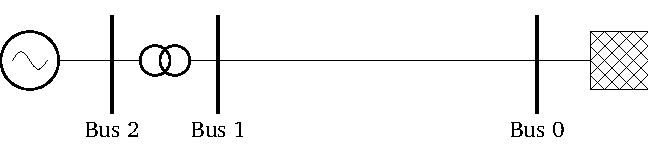
\includegraphics{tikz_graphics/images/smib_model.pdf}
    \vspace{12pt}
    \caption[Single line respresentation of the \acs{SMIB} model]{\acf{SMIB} model for verification and validation of the Python framework; own figure after \autocite{machowski_2020,kundur_2022}}
    \label{fig:smib-model}
\end{figure}

\begin{table}[htb]
    \caption[Simulation Setup for validation of the $\Pi$-modeled transformer]{Simulation Setup for validation of the $\Pi$-modeled transformer; considering a transforming ratio $\underline{\vartheta} \neq 1$ and $\underline{\vartheta} \in \mathbb{C}$}
    \label{tab:smib-model}
    \vspace*{12pt}
    \centering
    \small
    \begin{tabularx}{\textwidth}{Xr}
        % \toprule
        \textbf{Parameter} & \textbf{Value} \\ \hline
        \toprule
        Generator inertia $H$ & 3.5 s \\
        Generator damping $D$ & 0.1 p.u. \\
        Generator resistance $R$ & 0.01 p.u. \\
        Generator reactance $X$ & 0.1 p.u. \\
        Transformer resistance $R$ & 0.01 p.u. \\
        Transformer reactance $X$ & 0.1 p.u. \\
        Transmission line resistance $R$ & 0.01 p.u. \\
        Transmission line reactance $X$ & 0.1 p.u. \\
        \bottomrule
    \end{tabularx}
\end{table}

Further, this model shall be slightly modified according to \autoref{fig:smib-model-mod}. 
A load is added at the secondary bus of the transformer, the rest of the system is kept. \autoref{tab:smib-model} already contains this modification.

\begin{figure}[htb!]
    \centering
    \vspace{12pt}
    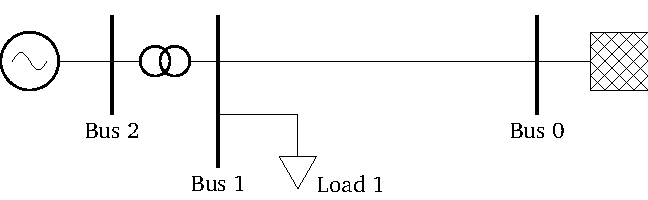
\includegraphics{tikz_graphics/images/smib_model_with_load.pdf}
    \vspace{12pt}
    \caption{Modified \acf{SMIB} model with additional load}
    \label{fig:smib-model-mod}
\end{figure}

\subsubsection{Simple Single Machine Load Model}

Following model is often recommended \quelle for easy voltage control studies, in explicit for \acsp{OLTC}. 
Similar to the \acs{SMIB} model, it consists from one synchronous generator, busses, and lines in a single branch. 
The \acs{IBB} is thus removed and changed to a load. 
This two element type o configuration allows for an easy analytical calculation of voltage stability and control. 
Although this thesis is focussing on \acs{OLTC} transformers, the model is extended with one in between. 
A single line representation is depicted in \autoref{fig:single-line-voltage-stability}.

\begin{figure}[htb!]
    \centering
    \vspace{12pt}
    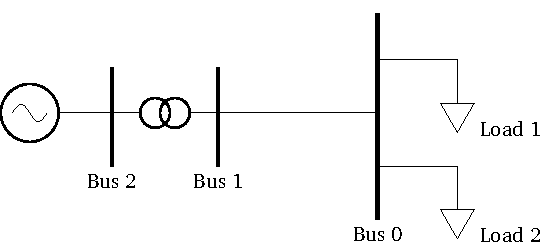
\includegraphics{tikz_graphics/images/sm_load_model.pdf}
    \vspace{12pt}
    \caption[Single line representation of a simple single machine load model]{Single line representation of a simple single machine load model; own illustration with characterstics from \quelle}
    \label{fig:single-line-voltage-stability}
\end{figure}

Further details about its configuration and simulation setup are included in \autoref{app:single-line-model}. 
It should be noted, that simple load models are not useful for simulation of this example network. 
Usually constant Z models are used as loads, therefore simulation results can be misleading and not showing desired effects or voltage instability mechanisms \quelle. 
% \commenting{The simulation framework is extended with XX types of load models, to satisfy the requirements of the single machine load model, and a connected stability assessment.}

% \subsubsection{IEEE Nine-Bus System}

% \subsubsection{Nordic Test System}

%%%%%%%%%%%%%%%%%%%%%%%%%%%%%%%
%%%%%%%%%%%%%%%%%%%%%%%%%%%%%%%
\section{Validation Steps}

Following section shall guide through the validation process.
Beginning with the new transformer $\Pi$-model, therefore lokking deeper into characteritic behavior dependent on the rated apparent power and the longitudinal ratio.
Proceeding with the three modeled control circuit and their behavior.
Lastly, some applied plausibilisations shall be done with the implemented voltage stability rating tools.

%%%%%%%%%%%%%%%%%%%%%%%%%%%%%%%
\subsection{Validation of the Modeled Transformer with Variable Tap Position}

As mentioned before, the base validation is concerning the basic transformer model.
For this, a parameter variation and comparison to the results from \textit{DIgSILENT PowerFactory} shall give a good representation of the accuracy.
The varied parameters are the apparent rated power $S_\mathrm{n}$ of the transformer, the longitudinal ratio $\vartheta$, the transformer reactance $X$, and the phase shifting angle $\phi$, resulting from the applied vector group.
The last two parameters are not included, because the transformer reactance is passively included in the ratio.
The reason for excluding the vector angle $\phi$ relies in the not congruent results.

\subsubsection{Variation of the Apparent Power}

\begin{figure}[htbp!]
    \centering
    \includegraphics[width=\linewidth]{development_files/validation/data/s_n_comp_errors.pdf}
    \caption[Model error comparison concerning the variation of the rated apparent power]{Absolute errors while comparing the tool \textit{diffpssi} with the software \textit{DIgSILENT PowerFactory}; One plot each for every parameter variation, concerning the errors for each bus}
    \label{fig:valid-s-errors}
\end{figure}

The rated apparent power $S_\mathrm{n}$ shall be varied in three steps acoording as described in \autoref{eq:variation-s-n}. 
The used grid model is the afore described \acs{SMIB} model. 
This is showing some predictable dynamics, but enabling a relative uncomplicated and easy to overview troubleshooting, if necessary.
The used grid parameters staying as described before, only the transformer apparent power is varied.
\begin{align}
    S_\mathrm{n} \in \{ 1100; 2200; 4400 \}~\mathrm{MVA} \label{eq:variation-s-n}
\end{align}
The used model for the comparative tool \textit{DIgSILENT PowerFactory} is as well included in the \textit{diffpssi} repository.
A plot of both results is depicted in \autoref{fig:valid-s-compl}
Looking deeper into one parameter, but plotting both tools in one diagram, \autoref{fig:valid-s-1100} in \autoref{app:add-validation-plots} is showing the results.
The three split diagrams account for each bus, where nearly no difference is obtainable.

Supporting this observation is the comparison of errors as illustrated in \autoref{fig:valid-s-errors}.
The error is not exceeding $0.005$ p.u. in any case.
One note to make here is, that due to the per unit nature of the calculation the initial values are often around $1$ p.u.
Therefore the seperate calculation of a relative error is neglected, as the absolute error is containing more information, and thus not surpassing the feel of relative nature.
Following this argumentation, the maximum relative error shall be around $0.05$ \% for this parameter variation.

\subsubsection{Variation of the Longitudinal Ratio}

\begin{figure}[htbp!]
    \centering
    \includegraphics[width=\linewidth]{development_files/validation/data/theta_comp_errors.pdf}
    \caption{Comparison of different varied parameters between \textit{diffpssi} and \textit{DIgSILENT PowerFactory}}
    \label{fig:valid-ratio-errors}
\end{figure}

In similar way as the validation approach for the rated apparent power, the longitudinal ratio shall be varied. 
Therefore the same network, with identical parameters is used, only that at this time the rated apparet power is fixed as well and the longitudinal ratio of the transformer is fixed during the simuatlion time according to following variation:
\begin{align}
    \vartheta \in \{ 0.9; 1.0; 1.1 \}~\mathrm{p.u} \label{eq:variation-ratio}
\end{align}
Looking into the results, in the same form as previously.
On the left side of \autoref{fig:valid-ratio-comp} is the result from the Python module \textit{diffpssi}, the right side is accounting for the validation tool \textit{DIgSILENT PowerFactory}.
The focussed comparison for the fixed ratio of $0.9$ p.u. is included in \autoref{app:add-validation-plots}.
As well \autoref{fig:valid-ratio-errors} is showing absoulte errors in the same manner.
The obtainable error for this case is comparably high, excluding for the reductive ratio of $0.9$ p.u.
This increasing with simulation time, to around a factor of 10 of the other errors. 
But still, this error is in a margin of lower than $1$ \%. 


%%%%%%%%%%%%%%%%%%%%%%%%%%%%%%%
\subsection{Parenthesis: Accountability of the Load Model}
\label{sec:validation-load-model}

\begin{figure}[htbp!]
    \centering
    \includegraphics[width=\linewidth]{development_files/validation/data/comparison_z_load.pdf}
    \caption[Comparison of the constant impedance model for each bus]{Comparison of the constant impedance model for each bus between the Python module \textit{diffpssi} and \textit{DIgSILENT PowerFactory}}
    \label{fig:z-comp}
\end{figure}

A static load model with quadratic dependency on the voltage had been implemented in the Python module before.
The load model can thus be classified as constant impedance model, or often referred as constant $\underline{Z}$ model \autocite{IEEELoadModeling_2022}. 
As this is playing a role in the chain of accumulating errors, following parenthesis shall give a feeling what contibution is generated through this load model.
For this evaluation the Single Line with Load model from \autoref{sec:networks} is used, with a load jump from $P=400\text{ MW}$ to $P=800\text{ MW}$ at the time stamp $1$ s.
The overall simulation time is set to $20$ s.
Other parameters are set as described in \autoref{sec:networks}.

\begin{figure}[htbp!]
    \centering
    \includegraphics[width=\linewidth]{development_files/validation/data/z_load_error.pdf}
    \caption[Absolute error comparison of the constant impedance model]{Absolute error of the already implemented constant impedance model over time; Accounted for both busses zero and one}
    \label{fig:z-load-error}
\end{figure}

\autoref{fig:z-comp} is showing the time series computation for each bus compared between both tools \textit{diffpssi} and \textit{DIgSILENT PowerFactory}.
Visible is the more extreme pronounciation of the overshoot and the convergence value over time of the Python package.
Looking at the absolute error comparison for each bus in \autoref{fig:z-load-error} showing a increase over time, and peak offsets of around $0.006$ p.u.
This accounts for an error lower than $1$ \% in this scenario.

%%%%%%%%%%%%%%%%%%%%%%%%%%%%%%%
\subsection{Validation of the OLTC Control Schemes}
\label{sec:validation-oltc-schemes}

To begin with this section of control scheme validation, the basic strategy accounted for all the considered models and verification setups.
The characterizations of the control loop feedbacks has already been carried out in the modeling chapter \autoref{sec:modeling-tap-changer-control}.
To validate the in-simulation behavior of the control loops, two different scenarios are accounted for the \acs{OLTC} and the \acs{FSM}.
First, the Simple Load against Machine grid is used with the declared parameters as in \autoref{sec:networks}.
To bring the system in a dynamic state, a load increase is added at the simulation time point $1$ s.
All differing values are pointed out in the validation result presentation later on.
Secondly, the more complex version of a \acs{SMIB} model with a connected load at the middle bus is used to account for a different scenario including a load flow direction change.
It would be expected, that neither \textit{DIgSILENT PowerFactory} or \textit{diffpssi} would be able to react on this supposed load flow direction change.

\subsubsection{Application of the Afore Described Logic}

The first consideration for validation of the \acs{OLTC} control is the simple load model against a machine.
The applied load change is shifting the real power of the load from $P=400\text{ MW}$ to $P=800\text{ MW}$ at the simulation time $1$ s.

\begin{figure}[htbp!]
    \centering
    \includegraphics[width=\linewidth]{development_files/validation/data/comp_oltc_simple-load.pdf}
    \caption[Time Domain Result of the OLTC control scheme applied on the extended \acs{SMIB} network]{\acf{TDS} of the standard discrete \acs{OLTC} control scheme; Result of the extended or modified \acs{SMIB} model with additional load}
    \label{fig:comp-oltc-simple}
\end{figure}

When comparing the time series solution from \autoref{fig:comp-oltc-simple} for both bus voltages, one can obtain a similar course of the curves. 
Nearly no deviation is visible, the tap changes of the \acs{OLTC} clearly visible and at the same times.
A similar picture is drawn, when loooking at the absolute error of this scenario in \autoref{fig:comp-oltc-error-simple}.
In the areas of time, where the switching occurs, peaks of errors are visible, showing just the numerical issues at the switching times.
After the half of the simulation time, a new (quasi-) stationary state is showing nearly no error.
This error is close to $0$ p.u., showing a even less error than previouly illustrated \autoref{sec:validation-load-model}.

\begin{figure}[htbp!]
    \centering
    \includegraphics[width=\linewidth]{development_files/validation/data/error_oltc_simple-load.pdf}
    \caption[Bus and Error Comparison for the standard discrete \acs{OLTC} scheme applied on the extended \acs{SMIB} model with load]{Comparison of the standard discrete \acs{OLTC} control scheme applied on the extended \acs{SMIB} model with additional load; One plot for each bus with data from \textit{diffpssi} and \textit{DIgSILENT PowerFactory}; Additional plot for showing the absolute error for each bus}
    \label{fig:comp-oltc-error-simple}
\end{figure}

Taking in consideration the second verification scenario, applying the discrete \acs{OLTC} control scheme to the extended \acs{SMIB} model with added load, one can obtain the \acs{TDS} visible in \autoref{fig:tds-oltc-ex-smib}.
For reasons of volume, this plot is just added to the appendix.
The added event at time step $1$ s is a load jump at bus 1 from $P=100\text{ MW}$ to $P=1100\text{ MW}$.
Comparing the results for each bus between the two tools \textit{diffpssi} and \textit{DIgSILENT PowerFactory} \autoref{fig:comp-oltc-control-ex-smib} is giving an overview.

\begin{figure}[htbp!]
    \centering
    \includegraphics[width=\linewidth]{development_files/validation/data/comp_oltc_ext-smib.pdf}
    \caption[Bus and Error Comparison for the standard discrete \acs{OLTC} scheme applied on the extended \acs{SMIB} model with load]{Comparison of the standard discrete \acs{OLTC} control scheme applied on the extended \acs{SMIB} model with additional load; One plot for each bus with data from \textit{diffpssi} and \textit{DIgSILENT PowerFactory}; Additional plot for showing the absolute error for each bus}
    \label{fig:comp-oltc-control-ex-smib}
\end{figure}

% Here, an interesting process is happening to the flow of power. 
% The load flow after the jump of the load at bus 1 is changing directions, from being primarly supplied from the machine at bus 2 and supplying the excess power to the grid coupling, to being primarly supplied by the external grid.
Two observations can be drawn, when looking at the evolution of the bus voltage magnitudes.
First, the tap changing of the \acs{OLTC} is not adressing the problem of letting the voltage drifting away.
The control is supporting the destabilization of the voltage at bus 2, and hence the connected machine.
Secondly, although the initial evolution of the voltages after the load increase event is showing similar results with small deviation between the two tools, the first \acs{OLTC} intervention is happening at a different time step.
All following ones are as well time shifted between the two tools, ending up with a absolute static offset voltage as in the previous scenario of nearly $0$ p.u.

\begin{figure}[htbp!]
    \centering
    \includegraphics[width=\linewidth]{development_files/validation/data/oltc_ex-smib_signals.pdf}
    \caption[Internal signals of the \acs{OLTC} control in the extended \acs{SMIB} model]{Internal signals of the \acs{OLTC} control in the extended \acs{SMIB} model; a) the longitudinal transformer ratio $u_\mathrm{l}$ or mathematically referred as $\vartheta$, b) the deadband filtered voltage difference signal $v_\mathrm{dead}$}
    \label{fig:int-signals-ext-smib-oltc}
\end{figure}

When looking deeper in the model and its signals, one can obtain, that the \acs{OLTC} control is thus switching correctly.
As displayed in \autoref{fig:int-signals-ext-smib-oltc}, the deadband flter is correctly surpassing just values greater than the deadband, otherwise zero.
As well as the longitudinal ratio on the other side, where distances of $5$ s are visible, consodering the time constant and the constant overshoot of the voltage difference of greater than the deadband, the control mechanisms seem to operate fine and plausible.

% \subsubsection{Found Discreptancies or Unexpected Behavior}

% \begin{figure}[htbp!]
%     \centering
%     \includegraphics[width=\linewidth]{development_files/validation/data/error_oltc_simple-load_discrep.pdf}
%     \caption[Discreptancy when looking at the validation of the simple load model with discrete \acs{OLTC} control]{Discreptancy when looking at the validation of the simple load model with discrete \acs{OLTC} control}
%     \label{fig:error-oltc-control-error-discrep}
% \end{figure}

% While looking into and analyzing the results from the tool \textit{DIgSILENT PowerFactory}, a strange interaction was found.
% \autoref{fig:error-oltc-control-error-discrep} is showing the error comparison between the same grid and events as firstly illustrated.
% The only change was the placement of the tap changer, respectively in which direction the ratio of the transformer was defined.
% In this case it was set to the \acs{LV} side of the transformer, while the comparing \textit{diffpssi} data was produced with a tap changer on the \acs{HV} side, the same data as before.
% \autoref{fig:comp-oltc-control-discrep} is showing the \acs{TDS} for this comparison.

% Unexpectedly and strangely, the error one can evaluate with this semantic false comparison is lower as the actual correct comparison.
% This is leading to the question of a relation to the wrong side in the modeling.
% But as described in the overall \autoref{sec:transformer-modeling}, exactly this consfusion had been marked as important and explained detailed.
% One further aspect is, that the occuring error with this additional model is now lower as the error with only the load model and parameter event considered, as displayed in \label{fig:z-load-error} from the previous subsection.

%%%%%%%%%%%%%%%%%%%%%%%%%%%%%%%
\subsection{Validation of the FSM Control Scheme}
\label{sec:validation-fsm-schemes}

The idea and proceeding of the validation of the \acs{FSM} is carryied out similar to the subsection before.
First, a simple load against machine model is used, with the same \mycomment[MK]{Sure the same?} parameters as described in \autoref{sec:networks}.
Extending this model, a second look into the extended \acs{SMIB} model is done.
Here the parameterization stays the same as well.

As described in the modeling chapter, specically \autoref{sec:modeling-tap-changer-control}, of the \acs{FSM} module control, two control methods are implemented.
First, as described in the paper of \textcite{burlakin_2024} with preferring the switching of the \acs{FSM}, and secondly the dependence on the function of tap skipping.
As only the last model is available in the comparative tool \textit{DIgSILENT PowerFactory}, only this can be compared and validated. 
The other control scheme is implemented similarly and used as well for futher studies.

\subsubsection{Voltage Difference Dependent Activation}

\begin{figure}[htbp!]
    \centering
    \includegraphics[width=\linewidth]{development_files/validation/data/tds_comp_fsm_simple.pdf}
    \caption[\acs{TDS} and error comparison for a \acs{FSM} control scheme based on the voltage difference applied on the extended \acs{SMIB} model]{\acs{TDS} and error comparison for a \acs{FSM} control scheme based on the voltage difference applied on the extended \acs{SMIB} model}
    \label{fig:tds-comp-fsm-vdiff-simple}
\end{figure}

\begin{figure}[htbp!]
    \centering
    \includegraphics[width=\linewidth]{development_files/validation/data/error_fsm_simple.pdf}
    \caption[\acs{TDS} and error comparison for a \acs{FSM} control scheme based on the voltage difference applied on the extended \acs{SMIB} model]{\acs{TDS} and error comparison for a \acs{FSM} control scheme based on the voltage difference applied on the extended \acs{SMIB} model}
    \label{fig:error-fsm-vdiff-simple}
\end{figure}

The first comparison, looking at the simple machine load model and the voltage dependent \acs{FSM} activation, \autoref{fig:tds-comp-fsm-vdiff-simple} is showing the bus wise comparison for the \acs{TDS}.
Nearly no spreading apart can be obtained, which is supported by \autoref{fig:error-fsm-vdiff-simple}.
This plot is showing the absolute error between \textit{diffpssi} and \textit{DIgSILENT PowerFactory}.
Each switching operation is sonnected with a short peak, approximately a numerical error.
After all possible switching operations took place, the statc error is settling around $0$ p.u., similar as all control scheme errors before.

\begin{figure}[htbp!]
    \centering
    \includegraphics[width=\linewidth]{development_files/validation/data/signals_ratio-k-m_fsm_vdiff.pdf}
    \caption[Internal signals for a \acs{FSM} control scheme switching dependent on the voltage deviation]{Internal signals for a \acs{FSM} control scheme switching dependent on the voltage deviation}
    \label{fig:signals-fsm-vdiff-ext-smib}
\end{figure}

Continuing with the extended \acs{SMIB} model and a load increase event from $P=100\text{ MW}$ to $P=700\text{ MW}$ at $1$ s, \autoref{fig:error-fsm-vdiff-simple} is showing the \acs{TDS} including the error comparison.
The switching events are clearly visible and around a similar time, although due to the more complex behavior not congruent.
The static offsets after a simulation time of $120$ s are converging to $0$ p.u. absolute error, while the peak errors are arond $0.1$ p.u.
These peak errors occur just for a short time and can be connected to the time shifted switching operations.

\begin{figure}[htbp!]
    \centering
    \includegraphics[width=\linewidth]{development_files/validation/data/error_comp_fsm_vdiff.pdf}
    \caption[\acs{TDS} and error comparison for a \acs{FSM} control scheme based on the voltage difference applied on the simple scenario]{\acs{TDS} and error comparison for a \acs{FSM} control scheme based on the voltage difference applied on the simple scenario}
    \label{fig:error-fsm-vdiff-simple}
\end{figure}

Looking deeper into the signal processing of the control scheme, one can obtain a beginning with the \acs{OLTC} as first acting part in \autoref{fig:signals-fsm-vdiff-ext-smib}.
The voltage difference is exceeding the deadband, but not large enough to activate the \acs{FSM} module yet.
Later on in the evolution the \acs{FSM} is gettinmg activated, but not dependent on the \acs{OLTC} switching or tap position.

\subsubsection{Preferring the FSM over the Normal OLTC}

\begin{figure}[htbp!]
    \centering
    \includegraphics[width=\linewidth]{development_files/validation/data/signals_ratio-k-m_fsm_pref.pdf}
    \caption[Internal signals for a \acs{FSM} control scheme preferring the \acs{FSM}]{Internal signals  for a \acs{FSM} control scheme preferring the \acs{FSM}}
    \label{fig:signals-fsm-preferred}
\end{figure}

For the simple load against machine model no different result to the afore presented could be found.
The less drastic increase in voltage magitude difference is reuslting in the same switching behavior and module activation as with the voltage dependent \acs{FSM} control.
Therefore the \acs{FSM} is acting just as an increase in switchable tap positions, resp. transformer ratio spread.

Accounting for the second validation set up, the same network is chosen as for the validation of the first \acs{FSM} control scheme.
The event magnitude is increased to a change from $P=100\text{ MW}$ to $P=1100\text{ MW}$.
Because no implemented version of this control was available for the tool \textit{DIgSILENT PowerFactory}, no comparison can be drawn.
The result, a \acs{TDS} as alternative to the afore illustrated behavior, can be evaluated through \autoref{fig:tds-fsm-preferred}, where one can clearly distinguish between the first four switches as related to the \acs{FSM}.
The magnitude is apparantly twice as big as the following switches.

When looking into the signal processing of this setup, \autoref{fig:signals-fsm-preferred} is illustrating this behavior.
The \acs{OLTC} tap switching mechanism is only activated after the \acs{FSM} is reaching one of its maximum positions.
Although this scenario is connected to a larger jump in power as event, and thus with a steeper ramp up of the bus voltages, one can obtaim from \autoref{fig:tds-fsm-preferred} that the preferred switching is not connected to this.
The bus voltage is exceeding the deadband clearly longer than $5$ s, this is the remaining criteria for activation of the \acs{OLTC}.
But the voltage is increasing until the tap skipping function is exceeded for the caracteristic time of the \acs{FSM}.
The switching behavior is thus not only differing in the preference of the tap changers, but as well how much voltage deviation is accepted until a tap change is induced. 

\begin{figure}[htbp!]
    \centering
    \includegraphics[width=\linewidth]{development_files/validation/data/fsm_deaf_band.pdf}
    \caption[Illustration of the deaf band with the FSM preferring FSM control scheme]{Illustration of the deaf band with the FSM preferring FSM control scheme}
    \label{fig:deaf-band}
\end{figure}

One quite interesting error in this switching logic is the problem of a deaf area between the deadband and $\Delta m \cdot v_\mathrm{db}$.
If the occuring event is causing a rise in voltage deviation between these two values, but not exceeding the limit, the \acs{FSM} control is not being activated.
Therefore no tap changing is occuring, and because the \acs{FSM} can not getting into any extreme position, the normal \acs{OLTC} control is not getting activated as well.
Therefore the tap changing transformer is not doing anything, and acting sort of \glqq deaf\grqq~to the voltage deviation in that band.
\autoref{fig:deaf-band} is illustrating such a scenario, with considering the extended \acs{SMIB} model, having a load increase at $1$ s from $P=100\text{ MW}$ to $P=700\text{ MW}$.

%%%%%%%%%%%%%%%%%%%%%%%%%%%%%%%
\subsection{Voltage Stability Rating Plausibility}

This subsection is looking at the implemented tools, helping to evaluate voltage stability.
Some parts ca be validates through external sources, others can just be tried to plausibilize with the obtainable and expected behavior. 

\subsubsection{Nose Curve Validation}

As previously illustrated in \autoref{sec:nose-curves}, the Nose Curve calculation for simple cases is congruent with the analytical calculation.
When looking at more complex cases, \textit{DIgSILENT PowerFactory} is providing such a voltage curve calculation tool as well.
When only scaling one load at a desired bus, with variation of the loads on considering a constant power relation $\tan \phi$, one can compare it to the proposed and impolemented algorithm in this thesis.
The desired network is the IEEE 9-bus network from \quelle.
Considering a variation of the load at bus five, with its constant power angle $\tan \phi = 0.4$, one can compare the solutions in \autoref{fig:comp-9bus-nose-curve}.
All other load stay consistent, so that the maximum power transfer is reached in both simulation environments at around $405$ MW.
An interesting observation can be drawn in the beginning of the curve, where \textit{DIgSILENT PowerFactory} is naturally starting at the initial load operational power.
Apart from that, the curves are congruent as well.

\begin{figure}[htbp!]
    \centering
    \includegraphics[width=\linewidth]{development_files/theoretical/plots/9bus_comp_b5.pdf}
    \caption[Comparison of Nose Curve generation between \textit{diffpssi} and \textit{DIgSILENT PowerFactory} for the IEEE 9-bus system]{Comparison of Nose Curve generation between \textit{diffpssi} and \textit{DIgSILENT PowerFactory} for the IEEE 9-bus system at bus 5; Load only scaled at bus 5 and with constant $\tan \phi = 0.4$}
    \label{fig:comp-9bus-nose-curve}
\end{figure}

\subsubsection{Extension of Nose Curves: Plausibility}

\sidenote{OLTC ratio dependent curves}
The next extensions in the interest are the intersection points with the different load models at the bus, the include of \acs{TDS}, and the insertion of tap position dependent characteristics.
\autoref{fig:oltc-nose-curve} is targeting the last mentioned point and illustrating in dashed red lines the different tap dependent nose curves of a simple load machin network from \autoref{sec:networks}.
The discrete possible tap ratios are defined as following set:
\begin{align}
    \boldsymbol{R} := \{0.9 + n \cdot 0.02\} \quad \forall~\{ n \in \mathbb{N}~\vert~0 \leq n \leq 10 \} \notag
\end{align}

\begin{figure}[htbp!]
    \centering
    \includegraphics[width=\linewidth]{development_files/voltage_stability/plots/nose_curves_with-oltc.pdf}
    \caption[Nose curves dependent on the tap changer ratio for a simple load network]{Nose curves dependent on the tap canger ratio for a simple load network}
    \label{fig:oltc-nose-curve}
\end{figure}

Clearly visible are these transformer ratios for an unloaded grid.
The evolution of all tap positions deviating from the initial, or normal tap position illustrated as blue line, can be described as equidistant.
Resulting in the same critical maximum loading of the grid, but at different voltages.
This could be expected, as this \acs{OLTC} is solely a longitudinal tap changes, with no phase shifting capabilities at all.
The maximum transferable power shall thus not be different, as the transformer alone cannont support any reactive power

\begin{figure}[htbp!]
    \centering
    \includegraphics[width=\linewidth]{development_files/voltage_stability/plots/nose_curve_tds_load.pdf}
    \caption{Nose Curve with added \acs{TDS} and the power of a constant impedance load dependent on the voltage as intersection point}
    \label{fig:nc-tds-load}
\end{figure}

\sidenote{TDS in a static plot}
When concerning the first two visualization extensions, the includation of a \acs{TDS} and the load behavior in the static plot, one can obtain the results from \autoref{fig:nc-tds-load}.
The more pale the scatter points get, the further the point is in time of the simulation.
The basis sceario for this figure is the simple grid model, with an continous linear load increase over time statrting at the ase load of $P=400\text{ MW}$ and $Q=0\text{ Mvar}$.
The load could then be described in dependence of the time $t$ as 
\begin{align}
    s(t) = s_0 + 80\text{ MVA} \cdot t \notag,
\end{align}
resulting in a maximum power of approx. $P=10^4\text{ MW}$ after the complete simulation time of $120$ s.
One important thing to note on this figure is the usage of machine controllers, explicitly a \ac{SEXS}, \ac{GOV}, and a \ac{PSS}.
The parameterization of these models is included in \autoref{tab:machine-controllers}.
The size of the machine is set to $2200$ MVA, while its power delivery is at $P=1998$ MW.


\begin{figure}[htbp!]
    \centering
    \begin{subfigure}[b]{.49\linewidth}
        \centering
        \includegraphics[width=\linewidth]{development_files/voltage_stability/plots/nose_cuve_small-machine.pdf}
        \subcaption{$2200$ MVA}
    \end{subfigure}
    \begin{subfigure}[b]{.49\linewidth}
        \centering
        \includegraphics[width=\linewidth]{development_files/voltage_stability/plots/nose_cuve_big-machine.pdf}
        \subcaption{$5 \cdot 2200$ MVA}
    \end{subfigure}
    \caption[Nose Curve and \acs{TDS} for a simple load system without machine controllers]{Nose Curve and \acs{TDS} for a simple load system; Considering a machine without controllers and continous load increase; Left side showing a machine with $2200$ MVA size, on the right five times the size}
    \label{fig:tds-nose-curve-machine-sizes}
\end{figure}

Now looking into the \acs{TDS} for a machine without controllers, and the grid with a simple, non-tapping transformer, \autoref{fig:tds-nose-curve-machine-sizes} is showing a comparison on machine sizes.
The voltage is noch not following the static solutions of the grid, because the mechanical torque at the machine is constant, the exciter voltage is not adapted either.
Hence, the voltage is breaking in, and falling faster, than the network is limiting.
The voltage dipping is slower or with a lower gradient on the power, if the machine is bigger.
If a tap changer would have been added to the network, the curve would follow the same course, with parallel shifted points, similar to the illustration in \autoref{fig:oltc-nose-curve}.
But here the limitations or maximum loading points of the network cannot be reached as well.

\subsubsection{Envelope Violation Index}

The following shall demontrate the usage of the \acf{TVI}, when a scenario is either stable or unstable.
Using a standard \acs{SMIB} from \autoref{sec:networks}, and a added short circuit event from the time step $1$ s untill either $1.1$ s for the stable scenario, and $1.17$ s for the unstable scenario.
Now one can calculate the \acs{TVI} of each bus, the \acs{CSI} of the overall system, and relate all busses to the average of the system.
Further, the time stamps, where the voltage envelope is cut, can be returned as well. 
The shwon envelope in \autoref{fig:env-stable} can be replaced by a set of \acs{FRT}-curves as well.

\begin{figure}[htbp!]
    \centering
    \includegraphics[width=\linewidth]{development_files/voltage_stability/plots/env_stable_example.pdf}
    \caption[Voltage envelope for a stable scenario]{Voltage envelope for a stable scenario}
    \label{fig:env-stable}
\end{figure}

The \acs{TVI} for bus one in the shown stable scenario is approx. $0.06$, regarding the instable scenario $5.2$.
The voltage envelope violation time could be calculated for the instable scenario for each exit of the envelope, if the voltage has been inside it the timestep before.
Regarding the \acs{CSI} for this system, it can be calculated to approx. $5.8$, where bus one is rougly as critical as the system, bus zero is less critical with a \acs{TVI} of around $3.9$, and bus two is the most critical with a value of $8.5$.
The \acs{IBB} in this scenario is connected to bus zero, the short circuit event on bus one is harmin the stability of the connected machine at bus two. 
Bus one itself is supplied and strongly connected with the \acs{IBB}, thus making the bus two, which is isolated during the fault, the most critical one.

\begin{figure}[htbp!]
    \centering
    \includegraphics[width=\linewidth]{development_files/voltage_stability/plots/env_instable_example.pdf}
    \caption[Voltage envelope for an instable scenario]{Voltage envelope for an instable scenario}
    \label{fig:env-instable}
\end{figure}

%%%%%%%%%%%%%%%%%%%%%%%%%%%%%%%
\section{Model Limitations and Improvements}

\sidenote{Transformer modeling}
Concluding either the model of the transformer and its control schemes, they both can be classified as valid in comparison to the commercial software \textit{DIgSILENT PowerFactory}.
For the given and illustrated parameters, this can be stated.
With the exception of a complex transformer ratio, meaning a phase shifting part, the results are in the expected range of error.
The control schemes show similar switching logic and times.
Although the connecting error chain must not be neglected, and depending on the application already a few percent alteration can make a huge difference.
For example a difference of one percent can become an error of ten percent, if the objected voltage band is $0.1$ p.u.

The reduction of the error in the \acs{TDS} from only assessing the load model to the addition of the \acs{OLTC} control schemes seems plausible.
The control scheme is holding the voltage closer to the reference value. 
The load model has the lowest error near the reference value.
The further apart, the bigger the error, so that the accumulation of errors over the simulation time gets limited with the addition of an \acs{OLTC} control scheme.

Regarding the slightly different switching behavior, especially with the more sensitive \acs{FSM} control can be argued with the dependence on a hand full of factors and errors.
As the system converges into a congruent steady state after the dynamics, it seems thus comparable.
Although it has to be kept in mind, that real switching times can differ, so that coincidences of switching at the right time have to be ruled out through slight variations for example.
Further from the two small differing \acs{FSM} control schemes can be deviated, that a significant differing behavior can result already from small tweaks.
Not every possible scenario can be catched or stabilized with a globalized control scheme, as every one is more likely to have its own very specific application.

% \commenting{
%     Points to address from the transformer and the control modeling:
%     \begin{itemize}[nosep]
%         \item Error chain and multiplication could be possible -> For the OLTC: Reducing the error of the load model is possible as well, because the voltage is longer held near the reference value, where the error of the load model is the smallest
%         \item Correct switching of the Control Schemes -> Bus Voltages look okay, althought they are not always identical -> too many small influences on that 
%         \item Already a small difference in the FSM control scheme makes a lot of difference in the behavior -> Control schemes will not satisfy every possible control target, unless they are not overall complicated or else
%     \end{itemize}
% }

\sidenote{Voltage evaluations}
Switching the perspective to the assessment of voltage stability, there are other conclusions.
On the one hand it becomes also visually clear, that static stable solutions considering the voltage of a power system are decoupled from the possible dynamics.
If the system has no perspective on finding a static stable convergent, the dynamics solely will not be stable as well, except supportive operating units can be activated in time.
The other way round, meaning having a stable possible convergent, does not mean that with neglecting the dynamics a stable convergent must be found.
Even for the network limitations compared to limitations on voltage stability from machines a similar scenario can be watched.
If the network can transmit the load at the necessary stable voltages, the machine could possibly run out of power reserves, so that unstability occurs.
The same way that a grid can limit the transmission of sufficient power, when the generation units are provide capabilities.
Thus the critical points can often lie beyond or above the voltage bands for certain power points, \acsp{OLTC} can help stabilizing this as a convergent, if they shift the power voltage curves in the right direction.
Looking at the size of the machines, a similar perspective can be drawn. 
Bigger machines help staying closer to the static solution set with the same rate of load change.
When now dynamics are starting to occur as well, the \acs{TVI} can help with the static solution set, and the evaluation of the machines, if the system is more or less likely to become stable compared to other scenarios.
The impact of \acsp{OLTC} on the static solutions can be estimated, even the dynamics can be compared to the static behavior.

% \commenting{
%     Points to address from the voltage stability monitoring:
%     \begin{itemize}[nosep]
%         \item Stiffness of the models via apparent power: Comparison of static solutions and Dynamic Behavior
%         \item Limitation from the machine level on voltage solution is seems plausible -> One can evaluate the contributions of machines on the voltage stability; if grid max can be surpassed it is a grid limitation
%         \item Visible jumps in the tap positions seems in the same range as predicted by the nose curves
%         \item Time series computations illustrate the correct power, but not necessary the network only solution -> Dependent on machines etc. and their dynamics as well
%         \item Envelope violations make the stability of the voltage comparable as in a dynamic aspect
%     \end{itemize}
% }

\section{Summary in Short and Simple Terms}

Summarizing this chapter, the modeled transformer implementation and therefore connected control schemes deliver similar and comparable results to the commercial software \textit{DIgSILENT PowerFactory}.
Although the solutions are not always congruent, they can be classified as absolutely valid.
Numerical errors, small modeling differences, or a different behavior of the surrounding simulation environment cause small deviations.
These do not hinder the significance and capailities of the extended tool \textit{diffpssi}.
Looking futher into the constructed tools for voltage stability analysis, these are showing partly congruent behavior with the software \textit{DIgSILENT PowerFactory} as well.
The other tools show functional behavior, making conclusive predictions, claims or statements.
They can thus be used to compare system states with regards to voltage stability expectations and voltage dynamics.